\documentclass{ximera}  
\title{Dynamic Programming}  
\begin{document}  
\begin{abstract}  
We give an introduction to dynamic programming techniques via examples.
\end{abstract}  
\maketitle

\section{Dynamic Programming}

In the Recursion section, we defined the Fibonacci sequence recursively as $$f_n=\begin{cases} 1 & \text{if $n=0,1$}\\ f_{n-1}+f_{n-2} & \text{otherwise.}\end{cases}$$ Additionally, we presented the following code to compute these values:
\begin{sageCell}
def fib(n):
        if n < 2:
                return 1
        else:
                return fib(n-1) + fib(n-2)			
fib(5)
\end{sageCell}
While the function for \verb|fib| is very short and easy to read, it does suffer from one major drawback. If you try to compute \verb|fib(100)| you will find that the computer will complain and not be able to do it. Why? Because to compute \verb|fib(100)|, the program will first attempt to compute \verb|fib(99)| before computing \verb|fib(98)| and adding those values together. But to compute \verb|fib(99)| it will first compute \verb|fib(98)| before computing \verb|fib(97)| and so on. So you can see that the program is giving the computer a lot of needless work. The program ends up computing the same values multiple times because it never ``remembers" that it already did the same work before. A better approach would be to start from the beginning and work our way up to the desired term in the sequence. We write down, in a list or table, the terms of the sequence as we compute them. If we ever need them again, we just look to our table of computed values rather than recomputing them (which can waste a lot of time). Below is an example of this approach:
\begin{sageCell}
def dyn_fib(n):
        if n < 2:
                return 1
        else:
                L = [0 for i in range(n)]
                L[0] = 1
                L[1] = 1
                for i in range(2,n):
                        L[i] = L[i-1]+L[i-2]
                return L[-1]
dyn_fib(100)
\end{sageCell}

What we are really doing here is trading computational time for space on your computer's memory. We spend less time computing the desired value by avoiding duplicate work, but we require enough space in memory to hold all of the values we may need. This is what is referred to as a dynamic programming approach. Dynamic programming can work well whenever you have a problem whose solution can be determined by first solving sub-problems of the same type and then combining those solutions to solve the original problem. In the case of the Fibonacci sequence, the value of $f_n$ is clearly related to prior values of the sequence, $f_{n-1}$ and $f_{n-2}$, when $n\geq 2$. (Note: We do not actually need dynamic programming for the Fibonacci sequence, but it makes for an easier example to use as an introduction.)

Once we decide to use dynamic programming to solve a problem, such solutions typically involve a few steps:
\begin{enumerate}
	\item We must create a list or table where each entry will contain the solution to some related sub-problem.
	\item We must populate the list with solutions to initial cases (for recursively defined functions this would be the base cases).
	\item We must determine what relationship exists between the list or table entries in order to populate the rest of the list without doing any duplicate work.
\end{enumerate}

In the case of the Fibonacci sequence, our second solution applied the above steps in the following way:
\begin{verbatim}
==============================
L is a list of length n

L[i] is ith Fibonacci number

L[0],L[1] = 1

L[i] = L[i-1] + L[i-2] for i >= 2
==============================
\end{verbatim}

\section{Examples}

In this section we illustrate how to use dynamic programming via several examples.

\subsection{The Lightbulb Problem}

Suppose that a company sells lightbulbs in packages of size 1, 2, 6, and 8. If a customer orders 30 lightbulbs, what is the least number of packages (of any size) that can be used to put this order together?

We begin with an simple approach. How many packages would we have to use if we simply tried using the largest package available at the time? In this case we would end up using 3 packages of size 8 and one of size 6. This is optimal here, but this strategy does not always work. (Try applying this same strategy to an order of 12 lightbulbs.)

To see how to use dynamic programming, let's work backwards. When putting an order of 30 lightbults together, we either:
\begin{enumerate}
	\item solved the problem for 22 bulbs and added a package of size 8, or 
	\item solved the problem for 24 bulbs and added a package of size 6, or 
	\item solved the problem for 28 bulbs and added a package of size 2, or 
	\item solved the problem for 29 bulbs and added a package of size 1.
\end{enumerate}
So if we could first solve the problem for 22, 24, 28, and 29, we could solve the problem for 30 by finding the minimum solution out of those 4 problems and adding 1 (for the additional package needed to get to 30). Working backwards this way we see that we would also need to solve some initial cases, namely 1 to 8 would do. So we will establish a list of values that will track our sub-problem solutions together with some initial cases and the relationship between entries in our list.
\begin{verbatim}
==============================
L is a list of length n

L[i] is the minimum number of packages 
     needed to put together a lightbulb order of size i

L[1] = 1, L[2] = 1, L[3] = 2, L[4] = 2, 
L[5] = 3, L[6] = 1, L[7] = 2, L[8] = 1

L[i] = min(L[i-8], L[i-6], L[i-2], L[i-1]) + 1 for i >= 9
==============================
\end{verbatim}

We apply the above algorithm in the SageCell below. Two notes are needed here. We use \verb|N = max(8,n)| in place of \verb|n| to avoid issues when \verb|n| is smaller than 8 and we add an extra item in our list since lists are zero-indexed in Python.

\begin{sageCell}
def bulb(n):
        N = max(8,n)
        L = [0 for i in range(N+1)]
        L[1] = 1
        L[2] = 1
        L[3] = 2
        L[4] = 2
        L[5] = 3
        L[6] = 1
        L[7] = 2
        L[8] = 1
        for i in range(9,N+1):
                L[i] = 1 + min(L[i-8], L[i-6], L[i-2], L[i-1])
        return L[n]
bulb(30)
\end{sageCell}

\subsection{Maze Solver}

Suppose we are given a rectangular ``maze" like the one below. Assume that we always start at the top left corner and always end at the bottom right corner. If we are only allowed to move down or to the right, how many different paths can we take to get to the end? Our goal is to count the number of distinct paths from the start to the end of the maze.

The number of distinct paths from the start to the end of this maze is 3.
\begin{center}
	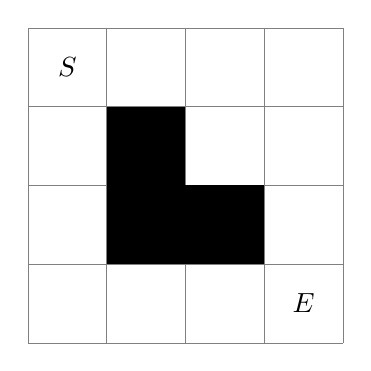
\begin{tikzpicture}[scale=1]
		\draw[help lines] (0,0) grid (4,4);
		\fill[black] (1,2) rectangle (2,3);
		\fill[black] (2,1) rectangle (3,2);
		\fill[black] (1,1) rectangle (2,2);
		\node at (0.5,3.5) {$S$};
		\node at (3.5,0.5) {$E$};
	\end{tikzpicture}
\end{center}

\noindent The 3 paths are give below.

\begin{figure}[h]
	\centering
	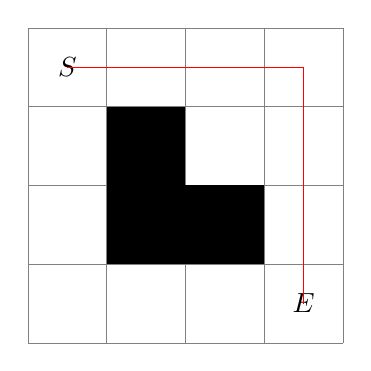
\begin{tikzpicture}[scale=1]
		\draw[help lines] (0,0) grid (4,4);
		\fill[black] (1,2) rectangle (2,3);
		\fill[black] (2,1) rectangle (3,2);
		\fill[black] (1,1) rectangle (2,2);
		\node at (0.5,3.5) {$S$};
		\node at (3.5,0.5) {$E$};
		\draw[red] (0.5,3.5) -- (3.5,3.5) -- (3.5,0.5);
	\end{tikzpicture}
	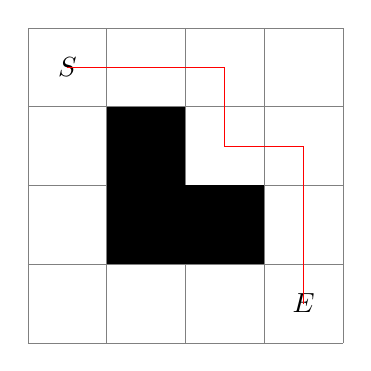
\begin{tikzpicture}[scale=1]
		\draw[help lines] (0,0) grid (4,4);
		\fill[black] (1,2) rectangle (2,3);
		\fill[black] (2,1) rectangle (3,2);
		\fill[black] (1,1) rectangle (2,2);
		\node at (0.5,3.5) {$S$};
		\node at (3.5,0.5) {$E$};
		\draw[red] (0.5,3.5) -- (2.5,3.5) -- (2.5,2.5) -- (3.5,2.5) -- (3.5,0.5);
	\end{tikzpicture}
	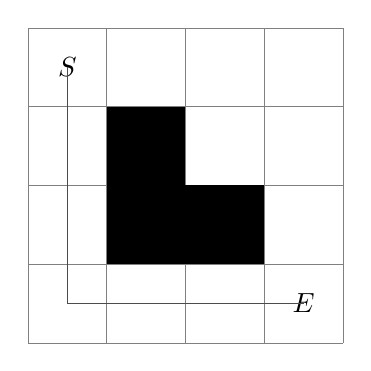
\begin{tikzpicture}[scale=1]
		\draw[help lines] (0,0) grid (4,4);
		\fill[black] (1,2) rectangle (2,3);
		\fill[black] (2,1) rectangle (3,2);
		\fill[black] (1,1) rectangle (2,2);
		\node at (0.5,3.5) {$S$};
		\node at (3.5,0.5) {$E$};
		\draw[red] (0.5,3.5) -- (0.5,0.5) -- (3.5,0.5);;
	\end{tikzpicture}
\end{figure}

In this problem, mazes are encoded as a list of lists where a 0 entry represents an open space in the maze and a -1 represents a blocked space in the maze. For example, the maze above is encoded as the following list:

\begin{verbatim}
==============================
maze = [[0, 0, 0, 0],
        [0,-1, 0, 0],
        [0,-1,-1, 0],
        [0, 0, 0, 0]]
==============================
\end{verbatim}

For each square in the maze, beginning with the start position, we count the number of ways you can enter the square if you can only move down and to the right.


\begin{enumerate}
	\item The following maze has 35 paths to the end.
\begin{verbatim}
==============================
[[0, 0, 0, 0, 0],
 [0, 0, 0, 0, 0],
 [0, 0, 0, 0, 0],
 [0, 0, 0, 0, 0]]
==============================
\end{verbatim}
	   \item The following maze has 52 paths to the end.
\begin{verbatim}
==============================
[[0, 0, 0,-1, 0, 0, 0, 0],
 [0,-1, 0, 0, 0, 0, 0, 0],
 [0, 0, 0, 0, 0, 0, 0, 0],
 [0,-1, 0,-1, 0, 0, 0, 0],
 [0,-1, 0, 0, 0, 0, 0, 0]]
==============================
\end{verbatim}
		

\subsection{The Longest Subsequence}



\subsection{The 0/1 Knapsack Problem}



\subsection{Minimum Insertions to Form a Palindrome}



\section{Problems}


\begin{question}
\end{question}

\section{Workspace}

\begin{sageCell}
# Use this cell to solve the above questions.
\end{sageCell}

\end{document}
